% !TEX root = ../main.tex
\section{System Model}
\label{sec:system-model}

% New section, 2026-10-17, at the owner's request: the systems engineering work
% gets its own section between the methodology and the experiment (D-028). Built
% from blocks moved whole, with their markers and source comments:
%   Stakeholders            <- 02_introduction.tex: Stakeholder Selection, the
%                              de-scoping part of Scope, Stakeholder Objectives
%   Constituent Systems     <- 02_introduction.tex: System Identification and Selection
%   System of Interest      <- 02_introduction.tex: the end of Scope and the context diagram
%   Operational Concept     <- 05_results_discussion.tex (now 06_)
%   Architecture            <- 05_results_discussion.tex (now 06_)
%   Proposed Airline-to-ATC Interface <- 03_assumptions_methodology.tex
% The Introduction keeps a short summary (Stakeholders and Study Boundary) that
% points here. The subsections run in order: who has a stake, what they want and
% where they conflict, which systems act, the boundary studied, how it operates,
% the architecture, and the interface the experiment tests.

\aidraft{Section opener, written 2026-10-17 for the new section. Replace with your own.}
This section presents the model the experiment is built on. It begins with the stakeholders, their objectives and the conflict among them, identifies the constituent systems through which they act, and draws the boundary of the System of Interest. It then describes how a flight operates within that boundary, the architecture that carries it, and the airline-to-ATC interface whose value the experiment of Section~\ref{sec:experiment} measures.
% ---- end AI draft

\subsection{Stakeholders}
\label{sec:stakeholders}

\subsubsection{Identification}

% Moved from the Introduction's Stakeholder Selection subsection, 2026-10-17.
Informed by the literature survey and the author's experience in the aviation industry, a set of candidate stakeholders was identified and refined using a PESTLE analysis and stakeholder discovery process. The result is a diverse group of stakeholders that represent the various interests and perspectives affected by NAS operational decisions, and is shown in Figures~\ref{fig:stakeholders-exploration} and~\ref{fig:stakeholders-power-interest}. The stakeholders are grouped by the six domains of a PESTLE analysis (political, economic, social, technological, legal, environmental) and scored for importance and impact on trajectory decisions. The assessment is documented in the \texttt{capstone\_stakeholder\_assessment.xlsx} file, along with an initial assessment of each candidate stakeholder's objectives, candidate MOPs and MOEs, and whether the stakeholder has a direct or indirect effect on trajectory decisions. The assessment also considers whether the stakeholder should stand alone or be abstracted through consolidation with another, and the reason for that decision. An excerpt of the work is in Appendix~\ref{app:stakeholders}, Table~\ref{tab:stakeholder-assessment-excerpt}.

\begin{figure}[htbp]
\centering
\figorbox{stakeholders_exploration.png}{MISSING: \texttt{report/figures/stakeholders\_exploration.png}}
\caption{Candidate stakeholders of the NAS as a system of systems.}
\label{fig:stakeholders-exploration}
\end{figure}

\begin{figure}[htbp]
\centering
\figorbox{stakeholders_impact_power_exploration.png}{MISSING: \texttt{report/figures/stakeholders\_impact\_power\_exploration.png}}
\caption{Candidate stakeholders placed by power and interest.}
\label{fig:stakeholders-power-interest}
\end{figure}
The power analysis informed the decision to keep four stakeholders in scope: the airline, air traffic control, the airport authority, and the flight crew. The other stakeholders are treated as boundary actors that supply rules, equipment, demand, and expectations to the decision but do not make it or execute it. The four kept stakeholders appear on the context diagram (Figure~\ref{fig:sysml-systemContext}) and are decomposed in the model.

\subsubsection{Candidate Objectives}

An exploration of each stakeholder's interests led to the following list of objectives relevant to the project:

% The descriptions were added 2026-10-17 at the owner's request ("add a brief
% description of the objectives to clarify what they are and why they're
% objectives"); the twelve names are the owner's list, unchanged.
\aidraft{One-line description of each objective: what it means in the NAS and which stakeholder holds it. Drawn from the per-stakeholder tables in \texttt{knowledge/models/stakeholder-objective-ontology.md} and the assessment spreadsheet; that file's own status note says its classifications are judgment calls not yet sourced from annotated literature, so these descriptions are too. The opening sentence on why each is an objective is Claude's.}
Each item is an objective because at least one stakeholder seeks to raise or lower it, and it can be measured, as a measure of performance for one system or a measure of effectiveness for the whole.
\begin{description}
    \item[Safety / Security] Keeping aircraft separated from each other, from terrain and from hazardous weather, and protecting the operation from deliberate harm. Held by every stakeholder; for air traffic control and the flight crew it is a constraint that is never traded.
    \item[Efficiency] Flying the flight with the least fuel and time for the distance covered. Held by the airline, whose fuel cost depends directly on the trajectory flown.
    \item[Throughput / Capacity] The number of aircraft a sector, runway or airport can handle in a period. Held by air traffic control and the airport authority.
    \item[Reliability / Resilience] The ability of the operation to run as planned and to recover when it is disrupted. Held by the airline and by air traffic control.
    \item[Environmental Impact] The carbon dioxide, other emissions and contrails a flight produces, which follow from the fuel it burns and the path it flies. Held by environmental and societal organizations and, through regulation, by governments.
    \item[Noise Impact] Sound over the communities near airports, set by the departure and approach paths. Held by communities and the airport authority.
    \item[Passenger Satisfaction] The passenger's experience of travel time, comfort and connections. Held by passengers, and by the airline through the revenue that follows.
    \item[Schedule Reliability] Arriving on time and keeping passengers' connections. Held by the airline and its passengers.
    \item[Cost / Profitability] The operator's cost of a flight (fuel, crew, the consequences of delay) and the profit it supports. Held by the airline and its investors.
    \item[Maintenance / Lifecycle Cost] The upkeep of aircraft and engines over their life. Held by the operator and the manufacturers.
    \item[Regulatory Compliance] Operating within the rules, procedures and clearances in force. Held by the flight crew and the airline, and enforced by the regulators.
    \item[Workload / Human Factors] The mental and procedural demand on controllers, dispatchers and crews. Held by air traffic control and the flight crew, for whom high workload is a cost and a source of error.
\end{description}
% ---- end AI draft
These objectives were then assessed for relevance to the decision under study, and six were kept: safety, efficiency, environmental impact, schedule reliability, cost, and workload. The other objectives were set aside for the reasons given in Section~\ref{sec:scope}.

\subsubsection{Selection}
\label{sec:scope}

% Moved 2026-10-17 from the Introduction's Scope subsection (the label sec:scope
% moved with it, so references to the de-scoping reasons still resolve). The
% closing sentence and the context diagram went to System of Interest below. One
% edit to the first sentence: it named the stakeholder and system subsections as
% coming before it; the systems now come after.
% Owner's note, 2026-10-11 print, page 7: "Leave larger list above, discuss
% de-scoping decisions here & include the final list/diagram." The strikes and
% margin notes on page 6 are the content below. Revised 2026-10-13 from the
% second print, pages 10 and 11: the kept stakeholders are named as on the context
% diagram, the reasons for profitability, reliability, maintenance and lifecycle
% cost and for throughput and capacity are the owner's handwritten ones, and the
% throughput call-out the owner scribbled over is removed.

\aidraft{De-scoping decisions and the final lists (owner's note: ``Leave larger list above, discuss de-scoping decisions here and include the final list/diagram''). The reasons in quotation marks are your margin notes. On the 2026-10-13 print you supplied the reasons for profitability, reliability, maintenance and lifecycle cost, and throughput and capacity; they are below in your words. Still Claude's reading, not yours: the reason given for the four stakeholders, and the reason given for security, resilience and regulatory compliance.}
The stakeholders and objectives above are the result of exploration. The study itself is narrower. It examines one tactical decision, the resolution of a conflict between aircraft in cruise, and keeps only the stakeholders and objectives that bear on that decision.

Four stakeholders remain, together with the aircraft, and each appears on the context diagram (Figure~\ref{fig:sysml-systemContext}): operators, as flight operations and its airline operations center; air traffic control, within airspace management; the airport authority, as airport operations; and the flight crew. The aircraft appears as aircraft systems. Governments and standards organizations, aircraft and engine manufacturers, passengers, and environmental and societal organizations are outside the System of Interest. They supply rules, equipment, demand, and expectations to the decision but do not make it or execute it, so they are treated as boundary actors and not decomposed.

Six stakeholder objectives remain: safety, efficiency, environmental impact, schedule reliability, cost, and workload. Schedule reliability is carried in the experiment as a step in cost when a flight's delay passes a threshold (the parameter $K$ of Section~\ref{sec:scoring-method}). The others were set aside for the following reasons. Noise impact: the measure is ``not relevant at cruise.'' Passenger satisfaction: ``not measurable objectively.'' Profitability falls out of the other objectives; it is tracked at the operator's organizational level and is more complex than any one decision. Reliability is captured with schedule reliability. Maintenance and lifecycle cost are largely determined by the number of flight cycles, the chosen takeoff performance, the flight distance and the climb controls, so one air traffic control decision has a negligible effect on them. Security, resilience and regulatory compliance are not changed by the choice between resolution options in the scenario. Throughput and capacity were left for another study. They are also close to ongoing work by the author, and out of an abundance of caution that part of the problem space was avoided.
% ---- end AI draft

\subsubsection{Objectives and Conflicts}
\label{sec:objectives-results}

% Drafted 2026-10-11 for the owner's note "DO" (print page 17) as a subsection of
% Results; moved to the Introduction 2026-10-13 (owner's note, print page 26: "Move
% to earlier section that discusses objectives?"); moved here 2026-10-17 as the
% close of Stakeholders, at the owner's suggestion. It follows Selection because it
% speaks only of the stakeholders and objectives kept there.
\aidraft{What ``optimal'' means to each stakeholder, and where the objectives conflict (your note: ``DO''). Source: the synthesis section of \texttt{knowledge/models/stakeholder-objective-ontology.md}, whose own status note says the classifications are judgment calls not yet sourced from annotated literature. Limited here to the stakeholders and objectives kept in Section~\ref{sec:scope}.}
Each stakeholder kept in scope pursues a different objective when an aircraft's trajectory is changed. The airline wants the lowest cost for its flights, which combines fuel, time, and the consequences of a late arrival for connecting passengers. Air traffic control wants separation assured with a workload the sector team can sustain, and a traffic picture that stays predictable. The flight crew wants instructions the aircraft can fly, given with enough time to set them up.

Some of these objectives align. Burning less fuel lowers the airline's cost and lowers carbon dioxide emissions together. Air traffic control's wish for predictability and the airline's wish to keep its schedule both favor aircraft that fly what was planned.

Others conflict, and the conflict this project studies is the first of them: the trajectory that is cheapest for one aircraft is not always the one that costs the sector least to grant. A request or a resolution that saves fuel for one flight can add instructions, monitoring, and follow-up for the controller. That cost is externalized. It does not appear in the airline's own cost function, and the party that bears it has no means to price it back.

The objectives also operate on different timescales. An airline sets its schedule policy over months, realizes fuel cost per flight, and realizes delay cost in minutes. Air traffic control manages capacity over years through sector design and over seconds through tactical control. A decision made in minutes by one party is judged against objectives the others hold on other clocks.
% ---- end AI draft

% Where to put the stakeholder requirements?

\subsection{Constituent Systems}
\label{sec:systems-selection}

% Was "System Identification and Selection" in the Introduction (made 2026-10-13
% from the owner's note on Figure 3, print page 9: "These are systems, not
% stakeholders. Move! 'System Identification & Selection'?"). Moved here and
% renamed 2026-10-17. The transition and the paragraph on the figure were added
% at the owner's request ("add a nice transition from the stakeholder work ...
% discuss the broad theorization reflected in the Miro board").
\aidraft{Transition from the stakeholder work, and a reading of the Miro board in Figure~\ref{fig:sos-exploration}. The description of the figure is Claude's reading of the exported image; the rationale the board reflects is the owner's and is only partly written down in the repository, so check each claim about why the board is drawn as it is.}
Stakeholders do not change a trajectory themselves. They act through systems: a controller through the sector's displays and radios, an airline through its operations center and dispatch tools, a crew through the flight deck and the flight management system. And the cost of whatever they decide is realized in one place, the aircraft, as fuel burned and time flown. The constituent systems through which the stakeholders act were therefore identified next.

Figure~\ref{fig:sos-exploration} places the NAS at the center and branches outward to the systems that could act on a flight: the aircraft, air traffic control, operators, airports, maintenance suppliers, communication, the regulatory bodies, and passengers. The board is deliberately broad. It follows the system-of-systems view quoted in Section~\ref{sec:introduction}, of many heterogeneous systems at several levels, and lists every system that could bear on a flight before any is set aside. Air traffic control divides into the air navigation service providers, whose terminal and en-route facilities control individual flights, and the national command center, whose traffic management units and flow programs shape demand across many. Operators divide into general aviation, airlines and militaries; within the airline, the operations center and its dispatchers sit beside the business, pilots, ticketing and IT functions.

The board decomposes its branches in two different ways, and the difference reflects the problem the project studies. The organizations that decide, air traffic control and the airline, are broken down to the people who make the decision: the individual controller and the dispatcher. The aircraft is broken down to the physical systems that carry it out: the flight management system's guidance and navigation functions, the propulsion components and the fuel system. The decision about a trajectory is made in one part of the system of systems, and its cost is realized in another.
% ---- end AI draft

\plantodo{Track C (owner's request, 2026-10-17)}{\textbf{Your experience behind the board.} Add what your experience in the FMS industry contributed to Figure~\ref{fig:sos-exploration} (an [SME] statement): for example, why the flight management system is decomposed to its functions, and which parts of the board came from that experience rather than from the literature of Section~\ref{sec:litreview}. Name any source the board drew on so it can be cited here.}

The aircraft is treated alongside the stakeholders as a constituent system. Figure~\ref{fig:sos-exploration} shows the systems first identified within the NAS, with the aircraft decomposed furthest, as its systems and their performance dictate the cost of each flight.

\begin{figure}[htbp]
\centering
\figorbox[\textwidth]{system_of_systems_detailed_exploration.png}{MISSING: \texttt{report/figures/system\_of\_systems\_detailed\_exploration.png}}
\caption{The NAS as a system of systems: candidate constituent systems.}
\label{fig:sos-exploration}
\end{figure}

\subsection{System of Interest}
\label{sec:soi}

% Made 2026-10-17. The closing sentence of the old Scope draft and the context
% diagram moved here from the Introduction.
\aidraft{Two connecting sentences, written 2026-10-17. They restate the selection of Section~\ref{sec:scope}; replace with your own.}
The System of Interest is drawn from the systems of Figure~\ref{fig:sos-exploration}: the systems operated by the four stakeholders kept in Section~\ref{sec:scope}, and the aircraft. The systems of the boundary actors are not decomposed; they appear only through what they supply to the decision.

Figure~\ref{fig:sysml-systemContext} is the resulting System of Interest as modeled: the constituent systems kept and the exchanges among them.
% ---- end AI draft

% GENERATED by tools/render_sysml_diagrams.py. Do not edit: the next run overwrites it.
% To change a caption, edit the `// caption:` line above the view in the .sysml file.
% To add or remove a figure, add or remove the view in the model.
% To move a figure between the body and the appendix, add or remove a
% `// placement: body` line above the caption line.

\begin{landscape}
\begin{figure}[!htbp]
\centering
\pdfimageresolution=300
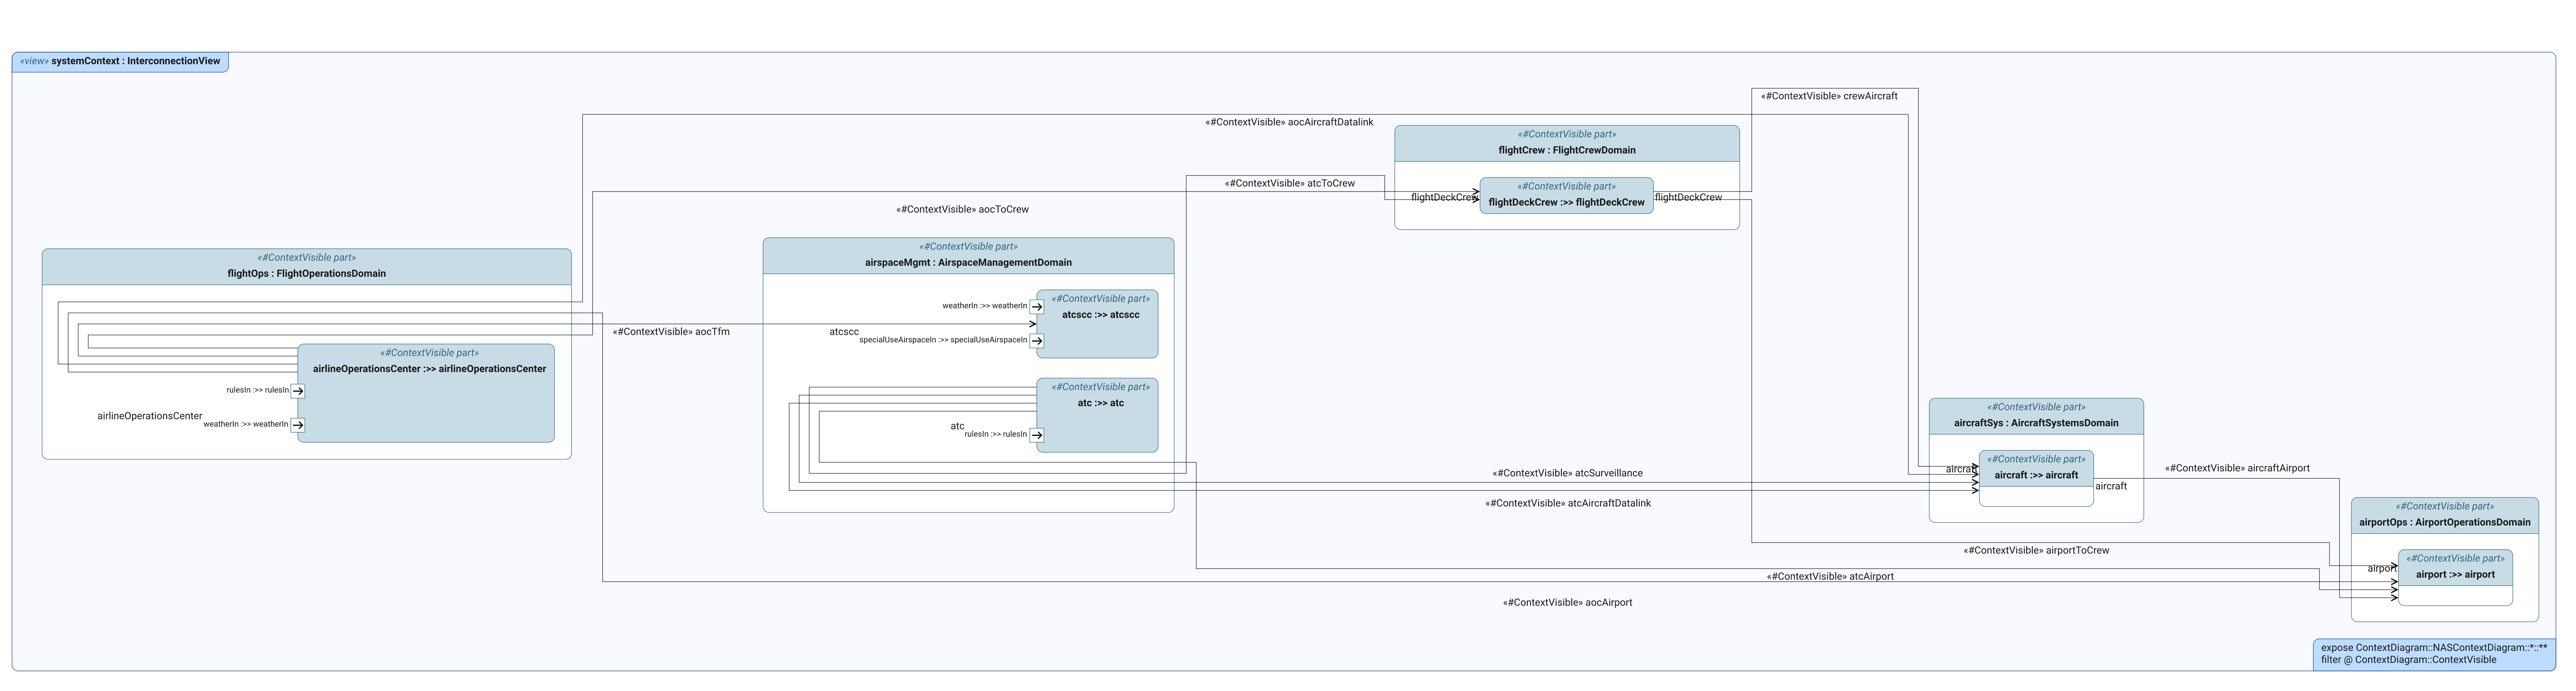
\includegraphics[width=\linewidth,height=0.8\textheight,keepaspectratio]{sysml/diagram-systemContext}
\caption{NAS context diagram. View \texttt{systemContext}; source \texttt{nas\_context\_diagram.sysml}; rendered 2026-10-10.}
\label{fig:sysml-systemContext}
\end{figure}
\end{landscape}


\subsection{Operational Concept}
\label{sec:conops-results}

% Moved 2026-10-17 from Results and Discussion, unchanged.
% Owner's notes, 2026-10-11 print, page 17: "DO"; "Show full detail 1st, then w/
% abstractions & provide rationale."; "The conops doesn't present my specific
% scenario. Need to update w/ the example conflict."
% The AI-DRAFTED call-out that stood here is removed (scribbled over on the
% 2026-10-13 print, page 24). Still true of the third paragraph: FlyEnroute is not
% yet decomposed in the model, so it describes where the conflict will sit, not
% what the diagram shows today.
The operational concept was first written in full detail as a gate-to-gate thread for one nominal commercial flight, from the pilot's point of view. It runs through eleven phases: the airline's schedule, fleet and crew assignment; the pilot's preparation before duty; reporting and the dispatch release; aircraft preflight and initialization of the flight management system; boarding, loading and fueling; clearance, pushback and taxi; takeoff and initial climb; climb; cruise; arrival planning; and descent through to the gate. Each phase records its initial state, the interfaces in use, and the questions it raised. The full thread is in Appendix~\ref{app:conops}.

The model carries an abstraction of that thread. Figure~\ref{fig:sysml-nominalOpsActivity} shows six actions in sequence: plan the flight, prepare for departure, depart, fly en route, arrive, and close out the flight. The eleven phases were reduced to six because the study concerns one decision in cruise. The phases before departure and after arrival fix the conditions that decision inherits (the aircraft's weight, its cost index, its schedule position) and are kept at the level needed to show where those conditions come from. Detail is added only where the studied decision is made.

The example conflict sits inside the fly en route action. Two aircraft in cruise are predicted to cross at the same level at the same time. The sector controller must move one of them, and each choice costs fuel, time and instructions that fall on different parties. The nominal thread treats a trajectory change in cruise as one step; the experiment of Section~\ref{sec:experiment} opens that step and asks what the decider knows when making it.

\plantodo{S5}{Decompose \texttt{FlyEnroute} one level in \texttt{nas\_activity\_diagram-nominal\_ops.sysml} so the conflict-resolution step appears on Figure~\ref{fig:sysml-nominalOpsActivity}, then check the three paragraphs above against the diagram. Put the full activity breakdown in Appendix~\ref{app:conops}.}

% GENERATED by tools/render_sysml_diagrams.py. Do not edit: the next run overwrites it.
% To change a caption, edit the `// caption:` line above the view in the .sysml file.
% To add or remove a figure, add or remove the view in the model.
% To move a figure between the body and the appendix, add or remove a
% `// placement: body` line above the caption line.

\begin{landscape}
\begin{figure}[!htbp]
\centering
\pdfimageresolution=300
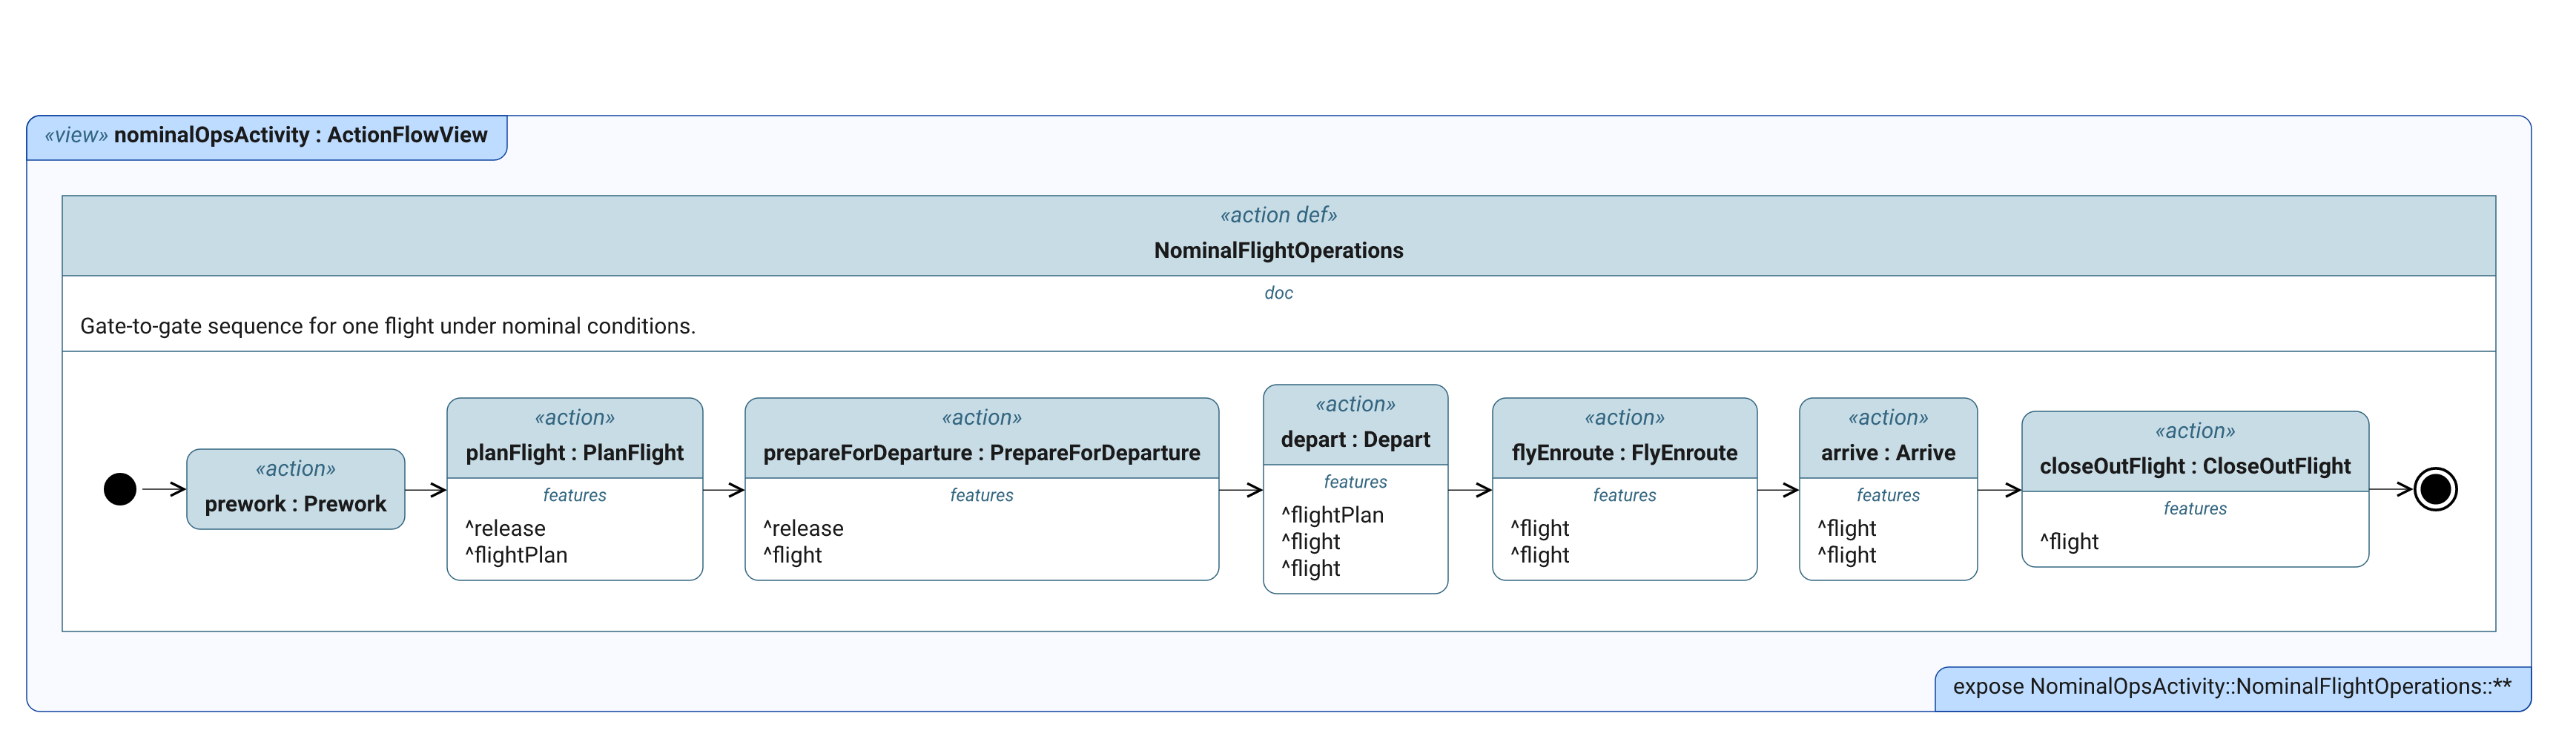
\includegraphics[width=\linewidth,height=0.8\textheight,keepaspectratio]{sysml/diagram-nominalOpsActivity}
\caption{Nominal flight operations activity diagram, phase level (each phase is decomposed in its own figure). View \texttt{nominalOpsActivity}; source \texttt{nas\_activity\_diagram-nominal\_ops.sysml}; rendered 2026-10-18.}
\label{fig:sysml-nominalOpsActivity}
\end{figure}
\end{landscape}


\subsection{Architecture: Detailed and Abstracted}
\label{sec:architecture-results}

% Moved 2026-10-17 from Results and Discussion, unchanged.
% Owner's note, 2026-10-11 print, page 17: "Place detailed & abstracted. Make sub-section."
\plantodo{S10}{Present the SysML architecture: package structure, the context diagram (Figure~\ref{fig:sysml-systemContext}), the internal block diagrams below, the interface and item-flow model, and the requirements model with traceability. For the aircraft, the detailed diagram comes first and the abstracted one second (your note: ``Place detailed and abstracted''); say what the abstraction drops and why. The airspace management diagram is still a placeholder.}

\aidraft{Two connecting sentences so the figures are referred to from the text. Replace with your own description of what each level of detail shows.}
The aircraft is shown at two levels of detail. Figure~\ref{fig:sysml-aircraftIbdDetail} is the detailed internal block diagram, including propulsion, airframe, landing gear, utilities, and the fuel and power links. Figure~\ref{fig:sysml-aircraftIbd} is the abstraction used in the rest of the report: the crew, the flight deck controls, the avionics, the flight controls, the fuel system, and the information and command links among them, which are the parts the studied decision passes through. Figure~\ref{fig:sysml-airspaceManagementIbd} shows the internals of airspace management as modeled so far.
% ---- end AI draft

% GENERATED by tools/render_sysml_diagrams.py. Do not edit: the next run overwrites it.
% To change a caption, edit the `// caption:` line above the view in the .sysml file.
% To add or remove a figure, add or remove the view in the model.
% To move a figure between the body and the appendix, add or remove a
% `// placement: body` line above the caption line.

\begin{landscape}
\begin{figure}[!htbp]
\centering
\pdfimageresolution=300
\includegraphics[width=\linewidth,height=0.8\textheight,keepaspectratio]{sysml/diagram-aircraftIbdDetail}
\caption{Aircraft internal block diagram, detailed level: adds propulsion, airframe, landing gear, utilities, and the fuel and power links. View \texttt{aircraftIbdDetail}; source \texttt{nas\_ibd\_aircraft.sysml}; rendered 2026-10-19.}
\label{fig:sysml-aircraftIbdDetail}
\end{figure}
\end{landscape}

% GENERATED by tools/render_sysml_diagrams.py. Do not edit: the next run overwrites it.
% To change a caption, edit the `// caption:` line above the view in the .sysml file.
% To add or remove a figure, add or remove the view in the model.
% To move a figure between the body and the appendix, add or remove a
% `// placement: body` line above the caption line.

\begin{landscape}
\begin{figure}[!htbp]
\centering
\pdfimageresolution=300

\includegraphics[width=\linewidth,height=0.8\textheight,keepaspectratio]{sysml/diagram-aircraftIbd}
\caption{Aircraft internal block diagram, default level of detail. View \texttt{aircraftIbd}; source \texttt{nas\_ibd\_aircraft.sysml}; rendered 2026-10-19.}
\label{fig:sysml-aircraftIbd}
\end{figure}
\end{landscape}

% GENERATED by tools/render_sysml_diagrams.py. Do not edit: the next run overwrites it.
% To change a caption, edit the `// caption:` line above the view in the .sysml file.
% To add or remove a figure, add or remove the view in the model.
% To move a figure between the body and the appendix, add or remove a
% `// placement: body` line above the caption line.

\begin{landscape}
\begin{figure}[!htbp]
\centering
\pdfimageresolution=300
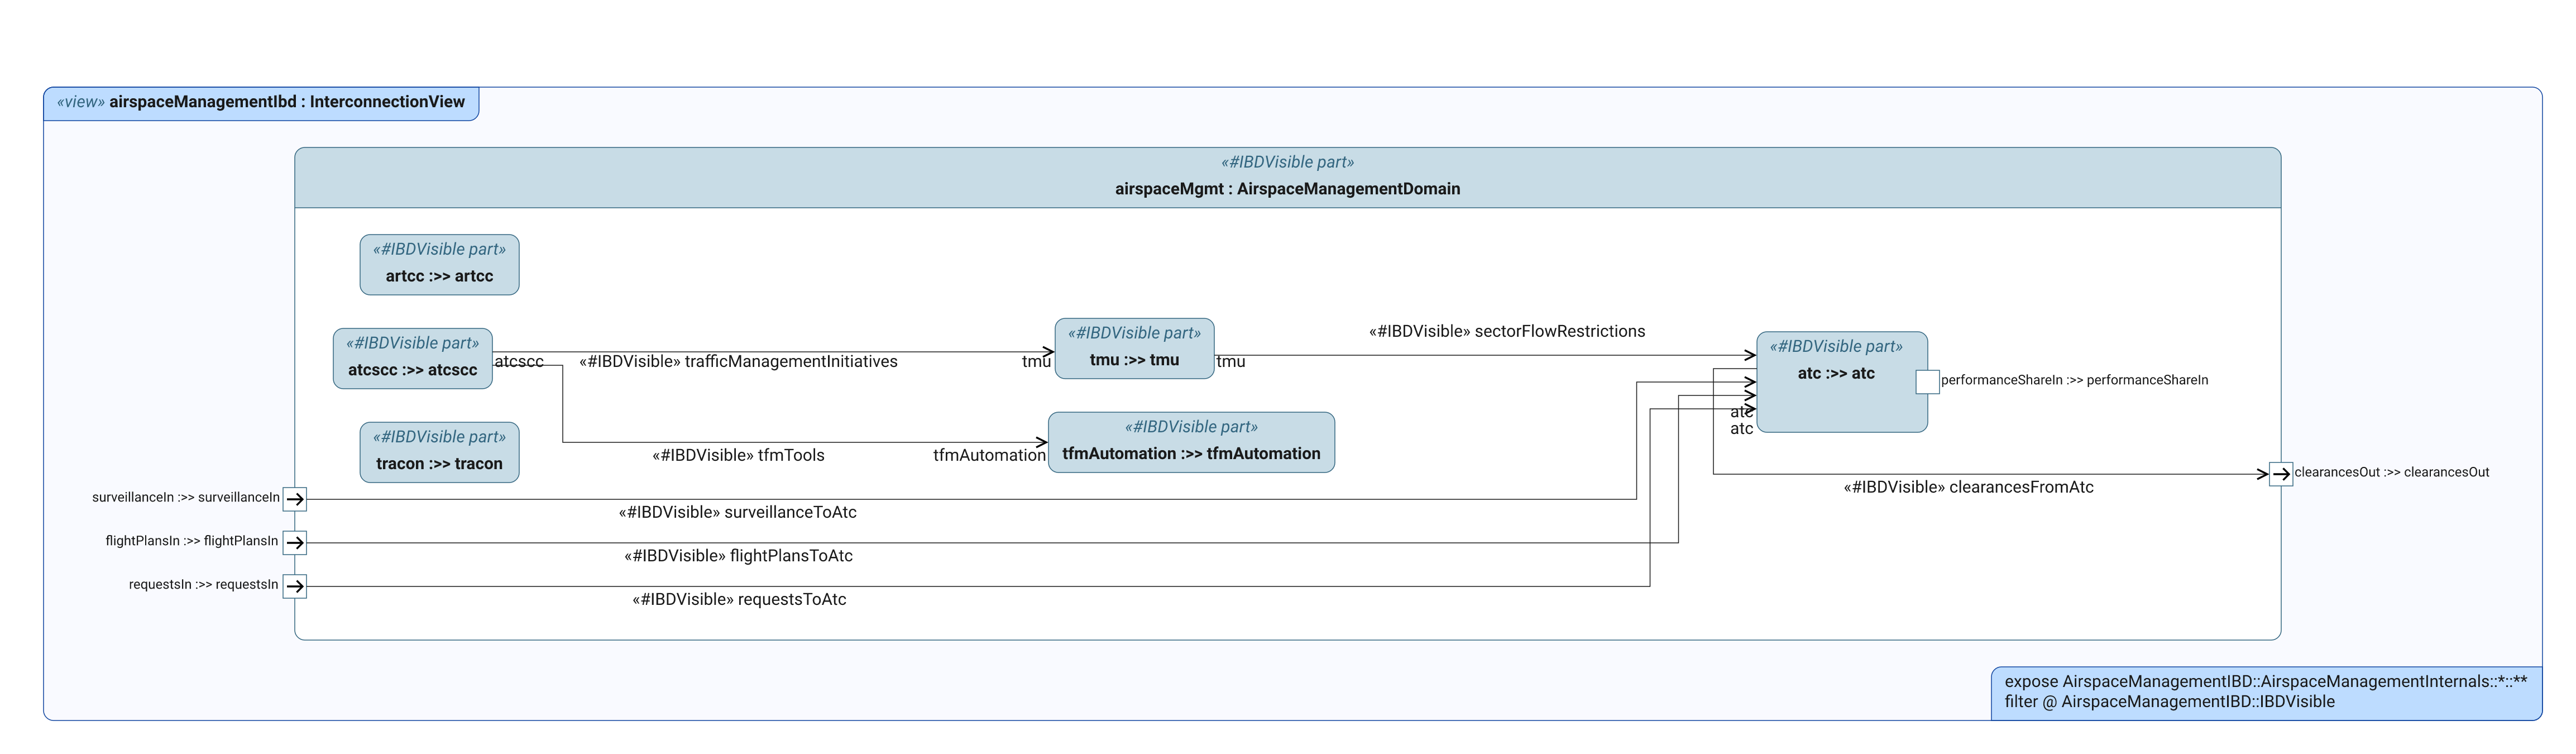
\includegraphics[width=\linewidth,height=0.8\textheight,keepaspectratio]{sysml/diagram-airspaceManagementIbd}
\caption{Airspace management internal block diagram. View \texttt{airspaceManagementIbd}; source \texttt{nas\_ibd\_airspace\_management.sysml}; rendered 2026-10-10.}
\label{fig:sysml-airspaceManagementIbd}
\end{figure}
\end{landscape}


\subsection{Proposed Airline-to-ATC Interface}
\label{sec:proposed-interface}

% Moved 2026-10-17 from Assumptions and Methodology. This answers the owner's
% question on the 2026-10-13 print, page 17 ("This shouldn't be its own section
% here. Where would this fit?"); that call-out is removed. The owner chose this
% place because the subsection leads into the experiment, which explores the
% interface's effect.
\plantodo{Track C (D-019)}{\textbf{Name the digital-thread artifact.} Describe \texttt{AirlinePerformanceShare}: what it carries (gross weight, cost index, connection priority; thrust, drag and fuel-flow model identifiers present but not exercised), who sends it (airline operations center or FMS), who receives it (ATC decision support, per D-012 owned by the system that decides), and which requirements it satisfies (SLR-INF-02) and the goal it serves (SLR-CLR-13). State that security is an assumption. \textbf{Owner's note, 2026-10-11 print: ``important to do''} --- position it against ADS-C EPP and Coppenbarger's Table 2 (the same items, a different receiver); a first draft of that positioning follows.}

% The AI-DRAFTED call-out that stood here is removed (scribbled over on the
% 2026-10-13 print, page 17); the owner's edits to the two paragraphs are applied.
% Still true of the second sentence: the ADS-C EPP statement rests on
% sesarju2019solutionsCatalogue, registered from its title page and contents only.
The items the interface carries are not new. \textcite{coppenbarger1999climbPrediction} listed take-off weight, thrust and drag factors, and the speed profile as candidates for exchange between an airline and air traffic control, and measured what airline-supplied weight does for the prediction of a climb. In Europe, the Extended Projected Profile is sent over ADS-C to downlink the trajectory that the flight management system predicts~\cite{sesarju2019solutionsCatalogue}. What has kept the items out of use is ownership, not feasibility: weight and speed intent ``are considered competitive parameters by airlines and are not available for use''~\cite{schultz2012adaptiveClimb}. A second obstacle is the availability of first-principles data for each aircraft type: thrust, drag and fuel flow.

The proposal here keeps the items and changes the receiver and the purpose. In the earlier work the data feeds a trajectory predictor, to make the prediction of one aircraft's flight path more accurate. Here it feeds the decision support of the party that chooses which aircraft to move, to change the choice. This provides for asking ``what if'' within a mathematical framework. The interface is typed in the model, tagged as part of the improved architecture, and tied to the requirement it satisfies, so the report can point at a model element where the earlier work has a finding in prose. Confidentiality is stated as an assumption: the data is disclosed only to the deciding party, and no security mechanism is modeled.

\aidraft{Closing link to the experiment, written 2026-10-17 (your note: the interface ``provides a good transition to the experiment, which will explore the impact of the new interface''). Replace with your own.}
The experiment that follows measures what this interface is worth. Its cases differ only in what the decider knows: in cases A and B the decider knows only what air traffic control knows today (the aircraft's type, level, speed and route, from which case B assumes a nominal weight), and in cases C and D it also has the items this interface carries. The difference between them is scored against the conflict of Section~\ref{sec:objectives-results}, at the level of the aircraft, the airline, the sector and the system.
% ---- end AI draft
